\documentclass[a4paper,12pt]{article}

\usepackage{mystyle}

\graphicspath{ {images/} }

\usetikzlibrary{arrows.meta}

\definecolor{my-red}{RGB}{176, 0, 0}
\definecolor{my-blue}{RGB}{0, 0, 153}


\author{Алексеев Василий}

%\title{Семинар 6}
%\date{13 + 19 октября 2020}
%
%\title{Семинар 7}
%\date{20 + 26 октября 2020}

\title{Семинар 8}
\date{27 октября + 2 ноября 2020}


\begin{document}
  \maketitle
  
  \tableofcontents

  \thispagestyle{empty}
  
  \newpage
  
  \pagenumbering{arabic}


  \section{Касательная к кривой второго порядка}
  
  Для эллипса, заданного в канонической системе координат уравнением
  \[
    \frac{x^2}{a^2} + \frac{y^2}{b^2} = 1
  \]
  уравнение касательной в точке $(x_0, y_0)$ эллипса выглядит так
  \[
    \boxed{\frac{xx_0}{a^2} + \frac{yy_0}{b^2} = 1}
  \]
  
  Для гиперболы, заданной в канонической системе координат уравнением
  \[
    \frac{x^2}{a^2} - \frac{y^2}{b^2} = 1
  \]
  уравнение касательной в точке $(x_0, y_0)$ гиперболы выглядит так
  \[
    \boxed{\frac{xx_0}{a^2} - \frac{yy_0}{b^2} = 1}
  \]
  
  И для параболы, заданной в канонической системе координат уравнением
  \[
    y^2 = 2px
  \]
  уравнение касательной в точке $(x_0, y_0)$ параболы выглядит так
  \[
    \boxed{yy_0 = p (x + x_0)}
  \]
  
  
  \subsection{\# 8.2(3)}
  
  Составить уравнение касательной к кривой
  \[
    xy = k
  \]

  \begin{solution}
    Можно продифференцировать обе части уравнения кривой в некоторой точке $(x_0, y_0)$, принадлежащей кривой:
    \[
      d(xy)\bigm|_{(x_0, y_0)} = d(k)
    \]
    Откуда
    \[
      x_0 dy + y_0 dx = 0 \Rightarrow \frac{dy}{dx} = -\frac{y_0}{x_0}
    \]
    То есть тангенс угла наклона касательной к кривой в точке $(x_0, y_0)$ равен $-\dfrac{y_0}{x_0}$.
    С другой стороны, тот же тангенс для касательной можно посчитать просто как отношение приращений $(y \hm- y_0)$ и $(x \hm- x_0)$ для некоторой точки $(x, y)$ касательной:
    \[
      \frac{y - y_0}{x - x_0} = -\frac{y_0}{x_0}
    \]
    
    Проводя упрощения и учитывая, что для исходной точки выполняется $x_0 y_0 \hm= k$, получаем
    \[
      y_0 x + x_0 y = 2k
    \]
  \end{solution}
  
  
  \subsection{\# 8.9(1)}
  
  Какие точки на кривой второго порядка
  \[
    \frac{27}{28} x^2 + \frac{9}{7} y^2 = 1
  \]
  удалены на наименьшее расстояние от прямой
  \[
    l\colon 3x + 4y + 5 = 0
  \]
  Найти это расстояние.
  
  \begin{solution}
    \begin{figure}[h]
      \centering

      \includegraphics[width=0.8\textwidth]{ellipse-8-9}
    
      \caption{Прямая $l$ не пересекает эллипс.}
      \label{fig:ellipse-8-9}
    \end{figure}
    
    Из рисунка (\ref{fig:ellipse-8-9}) видно, что прямая $l$ и эллипс не пересекаются, поэтому минимальное расстояние не нулевое.
    Также из рисунка понятно, что расстояние от точки $(x_0, y_0)$ эллипса до прямой $l$ будет минимальным в том случае, когда касательная к эллипсу в точке $(x_0, y_0)$ параллельна прямой $l$\footnote{Более строгое доказательство этого положения связано с тем, что эллипс выпуклый (отрезок, соединяющий любые две точки эллипса, лежит внутри эллипса) и что угол наклона касательной от точки к точке эллипса меняется непрерывно (то есть нет ``пропусков'' углов).}.
    Но таких точек, очевидно, у эллипса две (при этом если расстояние от одной из них до прямой $l$ будет минимальным, то от другой, наоборот, расстояние будет максимальным среди точек эллипса).
    
    Уравнение касательной к эллипсу в точке $(x_0, y_0)$:
    \[
      \frac{27}{28} x_0 x + \frac{9}{7} y_0 y = 1
    \]
    
    Сравнивая уравнение касательной с уравнением прямой, получаем условие параллельности касательной и прямой:
    \[
      \frac{27/28 x_0}{3} = \frac{9/7 y_0}{4}
    \]
    
    Откуда получаем
    \[
      x_0 = y_0
    \]
    
    При этом $(x_0, y_0)$~---~точка эллипса:
    \[
      \frac{27}{28} x_0^2 + \frac{9}{7} y_0^2 = 1
    \]
    
    В итоге
    \[
      \left\{
        \begin{aligned}
          &x_0 = \pm \frac{2}{3}\\
          &y_0 = \pm \frac{2}{3}
        \end{aligned}
      \right.
    \]
    
    Из рисунка (\ref{fig:ellipse-8-9}) видно, что подходит точка $\left(-\dfrac{2}{3}, -\dfrac{2}{3}\right)$.
    
    Расстояние от найденной точки до прямой $l$ в канонической системе координат эллипса (которая прямоугольная) вычисляется по формуле:
    \[
      \rho{\bigl((x_0, y_0), l\bigr)} = \frac{\left|3 \cdot \left(-\frac{2}{3}\right) + 4 \cdot \left(-\frac{2}{3}\right) + 5\right|}{\sqrt{3^2 + 4^2}} = \ldots = \frac{1}{15}
    \]
  \end{solution}
  
  
  
  \subsection{\# 8.24(1)}
  
  Составить уравнения касательных к эллипсу, заданному в канонической системе координат уравнением
  \[
    \frac{x^2}{18} + \frac{y^2}{8} = 1
  \]
  проходящих через точку $(-6, 0)$.
  
  \begin{solution}
    \begin{figure}[h]
      \centering

      \includegraphics[width=0.8\textwidth]{ellipse-8-24}
    
      \caption{Касательные к эллипсу, проходящие через одну точку на оси $X$ в канонической системе координат эллипса.}
      \label{fig:ellipse-8-24}
    \end{figure}
    
    Уравнение касательной к эллипсу в точке $(x_0, y_0)$, которая проходит через точку $(-6, 0)$ (\ref{fig:ellipse-8-24}):
    \[
      \frac{-6 x_0}{18} + 0 = 1 \Rightarrow x_0 = -3
    \]
    
    Подставляя найденную координату $x_0$ в уравнение эллипса, находим координаты $y_0$:
    \[
      \frac{(-3)^2}{18} + \frac{y_0^2}{8} = 1 \Rightarrow y_0 = \pm 2
    \]
    
    И уравнения касательных
    \[
      -2x \pm 3y - 12 = 0
    \]
  \end{solution}
  
  
  \subsection{\# 8.29(3)}
  
  Доказать, что пучок света, испущенный из фокуса параболы, отразившись от её стенок, пойдёт параллельно оси параболы.
  
  \begin{solution}
    \begin{figure}[h]
      \centering

      \includegraphics[width=0.5\textwidth]{parabola-8-29}
    
      \caption{Луч, исходящий из фокуса параболы.}
      \label{fig:parabola-8-29}
    \end{figure}
    
    Рассмотрим параболу в её канонической системе координат.
    Там она задаётся уравнением
    \[
      y^2 = 2px
    \]
    и уравнение касательной в точке $(x_0, y_0)$ будет
    \[
      y y_0 = p(x + x_0)
    \]
    или, если раскрыть скобки и перенести всё в одну часть уравнения
    \[
      p \cdot x - y_0 \cdot y + px_0 = 0
    \]
    Откуда получаем направляющий вектор касательной $\bds a \hm= (y_0, p)$ и вектор нормали к касательной
    \[
      \bds n \hm= (p, -y_0)
    \]
    
    Рассмотрим один луч, исходящий из фокуса параболы (\ref{fig:parabola-8-29}).
    Отраженный, по предположению, луч (параллельный оси параболы) параллелен вектору $\bds v_{\parallel} \hm= (-1, 0)$.
    Вектор же $\bds v$, ``по которому'' идёт испущенный из фокуса луч, равен $\left(x_0 \hm- \dfrac{p}{2}, y_0 \hm- 0\right)$.
    Найдём углы $\angle{(\bds v, \bds n)}$ и $\angle{\left(\bds n, \bds v_{\parallel}\right)}$.
    Если они окажутся равны, то мы докажем что требуется.
    Итак,
    \[
      \cos \angle{\left(\bds n, \bds v_{\parallel}\right)} = -\frac{p}{\sqrt{p^2 + y_0^2}}
    \]
    \[
      \cos \angle{(\bds v, \bds n)} = \frac{p \left(x_0 - \frac{p}{2}\right)^2 - y_0 y_0}{\sqrt{p^2 + y_0^2} \sqrt{\left(x_0 - \frac{p}{2}\right)^2 + y_0^2}} = \ldots = -\frac{p}{\sqrt{p^2 + y_0^2}}
    \]
    
    \medskip
    
    \emph{Небольшое замечание}: благодаря удачному выбору направления $\bds v_{\parallel}$ косинусы углов сразу получились равными.
    Но если бы $\bds v_{\parallel}$ был выбран как $(1, 0)$, то косинусы получились бы равными с точностью до знака (то есть просто по модулю).
  \end{solution}
  

  \section{Приведение уравнения кривой к каноническому виду}
  
  Общий вид уравнения кривой второго порядка:
  \begin{equation}\label{eq:second-order-curve}
    \left\{
      \begin{aligned}
        &Ax^2 + 2B xy + Cy^2 + 2Dx + 2Ey + F = 0\\
        &A^2 + B^2 + C^2 > 0
      \end{aligned}
    \right.
  \end{equation}
  
  Всего есть девять канонических уравнений кривых второго порядка\footnote{См., например книжку Беклемишева~Д.~В. или задачник.}:
  \begin{enumerate}
    \item\label{enum:ellipse} Эллипс
      \[
        \left\{
          \begin{aligned}
            &\frac{x^2}{a^2} + \frac{y^2}{b^2} = 1\\
            &a \geq b > 0
          \end{aligned}
        \right.
      \]
    \item ``Мнимый эллипс''
      \[
        \frac{x^2}{a^2} + \frac{y^2}{b^2} = -1
      \]
    \item ``Пара мнимых пересекающихся прямых''
      \[
        \frac{x^2}{a^2} + \frac{y^2}{b^2} = 0
      \]
    \item\label{enum:hyperbola} Гипербола
      \[
        \left\{
          \begin{aligned}
            &\frac{x^2}{a^2} - \frac{y^2}{b^2} = 1\\
            &a > 0,\ b > 0
          \end{aligned}
        \right.
      \]
    \item Пара пересекающихся прямых
      \[
        \frac{x^2}{a^2} - \frac{y^2}{b^2} = 0
      \]
    \item\label{enum:parabola} Парабола
      \[
        y^2 = 2px, \quad p > 0
      \]
    \item Пара параллельных прямых
      \[
        y^2 = a^2,\quad a \not= 0
      \]
    \item ``Пара мнимых параллельных прямых''
      \[
        y^2 = -a^2,\quad a \not= 0
      \]
    \item Пара совпавших прямых
      \[
        y^2 = 0
      \]
  \end{enumerate}
  
  Чтобы привести кривую к каноническому виду, можно придерживаться следующего алгоритма:
  \begin{enumerate}
    \setcounter{enumi}{-1}
    \item Перейти к прямоугольной системе координат (если она ещё не прямоугольная)\footnote{В задачах изначальная система координат будет считаться прямоугольной, если не сказано противное!}.
    \item \emph{Повернуть} систему координат так, чтобы исчез член с произведением $xy$.
    \item Далее, в зависимости от ситуации, надо \emph{перенести начало} системы координат так, чтобы исчезли либо линейные члены, либо свободный член.
    \item И в конце, опять же в зависимости от ситуации, может потребоваться ещё одно-два небольших действия, например изменение порядка координат (чего можно достичь поворотом на $\dfrac{\pi}{2}$, чтобы не менялась ориентация базиса).
  \end{enumerate}
  
  Центром кривой второго порядка называется точка $(x_0, y_0)$, такая что
  \[
    F(x_0 + \alpha, y_0 + \beta) = F(x_0 - \alpha, y_0 - \beta)
  \]
  где $F(\cdot, \cdot) \hm= 0$~---~уравнение кривой, а $\alpha$ и $\beta$~---~любые числа.
  Можно показать, что центр симметрии кривой~---~это почти то же самое, что и её центр (только центр в некоторых случая может существовать, а центр симметрии~---~нет).
  Если подставить в уравнение (\ref{eq:second-order-curve}) сдвинутые на $\pm \alpha$ и $\pm \beta$ координаты $(x_0, y_0)$ и приравнять, как в определении центра, то получим
  \[
    \alpha (Ax_0 + Bx_0 + D) + \beta (Bx_0 + Cy_0 + E) = 0
  \]
  откуда система уравнений для нахождения координат центра:
  \begin{equation}\label{eq:second-order-curve-center}
    \left\{
      \begin{aligned}
        &Ax_0 + Bx_0 + D = 0\\
        &Bx_0 + Cy_0 + E = 0
      \end{aligned}
    \right.
  \end{equation}
  
  Центр существует и единствен, если определитель системы отличен от нуля:
  \[
    \delta = \begin{vmatrix}A & B \\ B & C\end{vmatrix} \not= 0
  \]
  В этом случае кривая называется \emph{центральной}.
  
  При этом $\delta \hm> 0$ соответствует кривым эллиптического типа: от эллипса до гиперболы в списке кривых (\ref{enum:ellipse}),~---~$\delta \hm< 0$ соответствует кривым гиперболического типа: от гиперболы до параболы в списке кривых (\ref{enum:hyperbola}),~---~и $\delta \hm= 0$ соответствует кривым параболического типа: от параболы и далее (\ref{enum:parabola}).


  \subsection{\# 9.4(1)}
  
  Определить тип кривой второго порядка.
  Составить её каноническое уравнение и найти каноническую систему координат.
  Изначально кривая задана в \emph{прямоугольной системе координат}.
  \begin{equation}\label{eq:problem-9-4}
    F(x, y) = 2x^2 - 4xy + 5y^2 + 8x - 2y + 9 = 0
  \end{equation}
  
  \begin{solution}
    \vphantom{}
  
    \emph{Способ I (``канонический'')}.
    
    Тип кривой можно определить либо сразу, либо в самом конце, когда получим каноническое уравнение.
    Давайте отложим на конец (а в другом варианте решения сделаем это сразу).
    
    Первый шаг~---~надо повернуть систему координат так, чтобы исчез член со смешанным произведением переменных $xy$.
    Поворот системы координат:
    \[
      \left\{
        \begin{aligned}
          &x = x' \cos \phi - y' \sin \phi\\
          &y = x' \sin \phi + y' \cos \phi
        \end{aligned}
      \right.
    \]
    
    Подставляем в исходное уравнение и смотрим, что получается как коэффициент при $x'y'$:
    \begin{equation*}
    \begin{split}
      F'(x', y') &= 2 (x' \cos \phi - y' \sin \phi)^2 - 4 (x' \cos \phi - y' \sin \phi) (x' \sin \phi + y' \cos \phi)\\
      &+ 5 (x' \sin \phi + y' \cos \phi)^2 + \ldots
      = (6 \sin\phi \cos\phi - 4 \cos^2 \phi + 4\sin^2 \phi)x' y' + \ldots = 0
    \end{split}
    \end{equation*}
    Откуда получаем условие на угол поворота $\phi$, чтобы коэффициент при $x'y'$ обратился в ноль:
    \[
       3 \sin 2\phi - 4 \cos 2\phi = 0 \Rightarrow \tg 2\phi = \frac{4}{3}
    \]
    
    \begin{figure}[h]
      \centering

      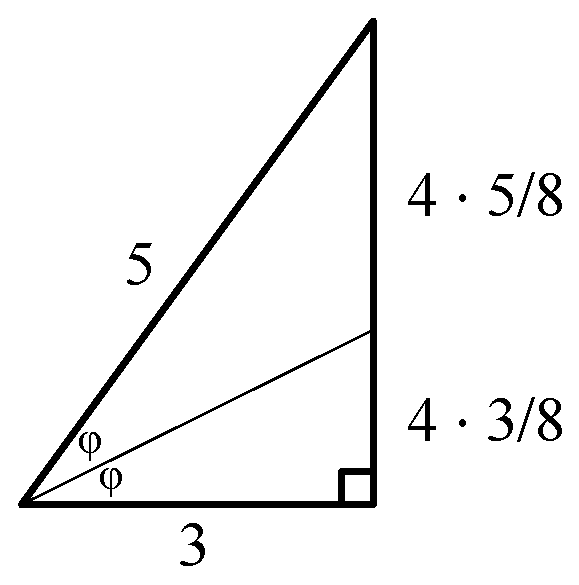
\includegraphics[width=0.25\textwidth]{triangle-9-4}
    
      \caption{К нахождению $\sin\phi$ и $\cos\phi$ по $\tg{2\phi}$.}
      \label{fig:triangle-9-4}
    \end{figure}
    
    Из рисунка (\ref{fig:triangle-9-4}), например, можно найти синус и косинус для одинарного угла:
    \[
      \left\{
        \begin{aligned}
          &\sin\phi = \frac{1}{\sqrt{5}}\\
          &\cos\phi = \frac{2}{\sqrt{5}}
        \end{aligned}
      \right.
    \]
    и первая замена
    \[
      \boxed{
        \left\{
          \begin{aligned}
            &x = \frac{2}{\sqrt{5}} x' - \frac{1}{\sqrt{5}} y'\\
            &y = \frac{1}{\sqrt{5}} x' + \frac{2}{\sqrt{5}} y'
          \end{aligned}
        \right.
      }
    \]
    
    Снова подставляем это представление $x$ и $y$ через $x'$ и $y'$ в исходное уравнение, но на этот раз выписываем все члены, кроме $x'y'$ (так как он обязан занулиться при замене $x, y$ на $x', y'$)
    \[
      F'(x', y') = \ldots = x'^2 + 6y'^2 + \frac{14x'}{\sqrt{5}} - \frac{12y'}{\sqrt{5}} + 9 = 0
    \]
    
    Далее можно выделить полные квадраты, чтобы избавиться от линейных членов
    \[
      \left(x'^2 + 2 \cdot \frac{7}{\sqrt{5}} x' + \frac{49}{5}\right) - \frac{49}{5}
        + \left(\left(\sqrt{6} y'\right)^2 - 2 \cdot \sqrt{6} y \cdot \frac{6}{\sqrt{30}} + \frac{36}{30}\right) - \frac{36}{30} + 9 = 0
    \]
    \[
      \left(x' + \frac{7}{\sqrt{5}}\right)^2 + \left(\sqrt{6} y' - \frac{6}{\sqrt{30}}\right)^2  = 2
    \]
    \[
      \left(x' + \frac{7}{\sqrt{5}}\right)^2 + 6\left(y' - \frac{1}{\sqrt{5}}\right)^2  = 2
    \]
    
    Откуда видна следующая замена\footnote{Множитель $6$ вынесен за скобку с $y'$ намеренно!}:
    \[
      \boxed{
        \left\{
          \begin{aligned}
            &x'' = x' + \frac{7}{\sqrt{5}}\\
            &y'' = y' - \frac{1}{\sqrt{5}}
          \end{aligned}
        \right.
      }
    \]
    
    Уравнение при этом в переменных $x''$, $y''$ примет вид:
    \[
      x''^2 + 6y''^2 = 2
    \]
    или, уже каноническое:
    \[
      \frac{x''^2}{2} + \frac{y''^2}{1/3} = 1
    \]
    
    Видно, что крива второго порядка~---~эллипс.
    Осталось задать каноническую систему координат, связав её и исходной.
    Надо вывести замену $x$ и $y$ сразу на $x''$ и $y''$, тогда станет известна матрицы перехода от исходного базиса к новому и положение новой (канонической) системы координат относительно исходной.
    
    Выражая и подставляя из одной замены в другую, получаем
    \[
      \left\{
        \begin{aligned}
          &x = \ldots = \frac{2}{\sqrt{5}}x'' - \frac{1}{\sqrt{5}}y'' - 3\\
          &y = \ldots = \frac{1}{\sqrt{5}}x'' + \frac{2}{\sqrt{5}}y'' - 1
        \end{aligned}
      \right.
    \]
    
    Откуда видны компоненты новых базисных векторов в старом базисе и положение нового начала:
    \[
      \left\{
        \begin{aligned}
          &\bds e_1' = \left(\frac{2}{\sqrt{5}}, \frac{1}{\sqrt{5}}\right)\\
          &\bds e_2' = \left(-\frac{1}{\sqrt{5}}, \frac{2}{\sqrt{5}}\right)\\
          &O'(-3, -1)
        \end{aligned}
      \right.
    \]
    
    
    \emph{Способ II (``через центр'')}.
    
    Если у кривой есть центр, то удобнее начинать замены с переноса начала координат в этот центр.
    Из системы уравнений (\ref{eq:second-order-curve-center}) можно понять, есть у кривой центр или нет
    И, если есть, найти его координаты
    \[
      \left\{
        \begin{aligned}
          &2x_0 - 2y_0 + 4 = 0\\
          &-2x_0 + 5y_0 - 1 = 0
        \end{aligned}
      \right.
    \]
    
    Определитель системы
    \[
      \delta = \begin{vmatrix}2 & -2 \\ -2 & 5\end{vmatrix} = 6 > 0
    \]
    (из того, что определитель больше нуля, сразу можно заключить, что кривая эллиптического типа).
    Решая далее, например, по методу Крамера, находим
    \[
      \left\{
        \begin{aligned}
          &x_0 = -3\\
          &y_0 = -1
        \end{aligned}
      \right.
    \]
    
    И первая замена~---~перенос начала координат в центр:
    \[
      \left\{
        \begin{aligned}
          &x = x' - 3\\
          &y = y' - 1
        \end{aligned}
      \right.
    \]
    
    Подставляя в уравнение (\ref{eq:problem-9-4}), получаем
    \[
      2x'^2 + 5y'^2 - 4x'y' = 2
    \]
    то есть линейные члены ушли.
    Осталось повернуть систему координат.
    Поворот должен быть таким же, как в первом способе решения.
    И в итоге
    \[
      x''^2 + 6y''^2 = 2
    \]
    
    Получили то же самое, что и в первый раз, но вычислений пришлось проводить в разы меньше (и вероятность совершить какую-нибудь ошибку тоже меньше).
    И координаты нового центра стали известны уже на стадии первой замены переменных.
  \end{solution}
  
  \newpage
  
  
  \section{Дополнение}
  
  \subsection{Про конические сечения}
  
  Кривые второго порядка можно получать, пересекая двойной круговой конус (не обязательно прямой) плоскостью, не проходящей через вершину конуса (\ref{fig:conic_sections}).
  
  \begin{figure}[h]
    \centering
    
    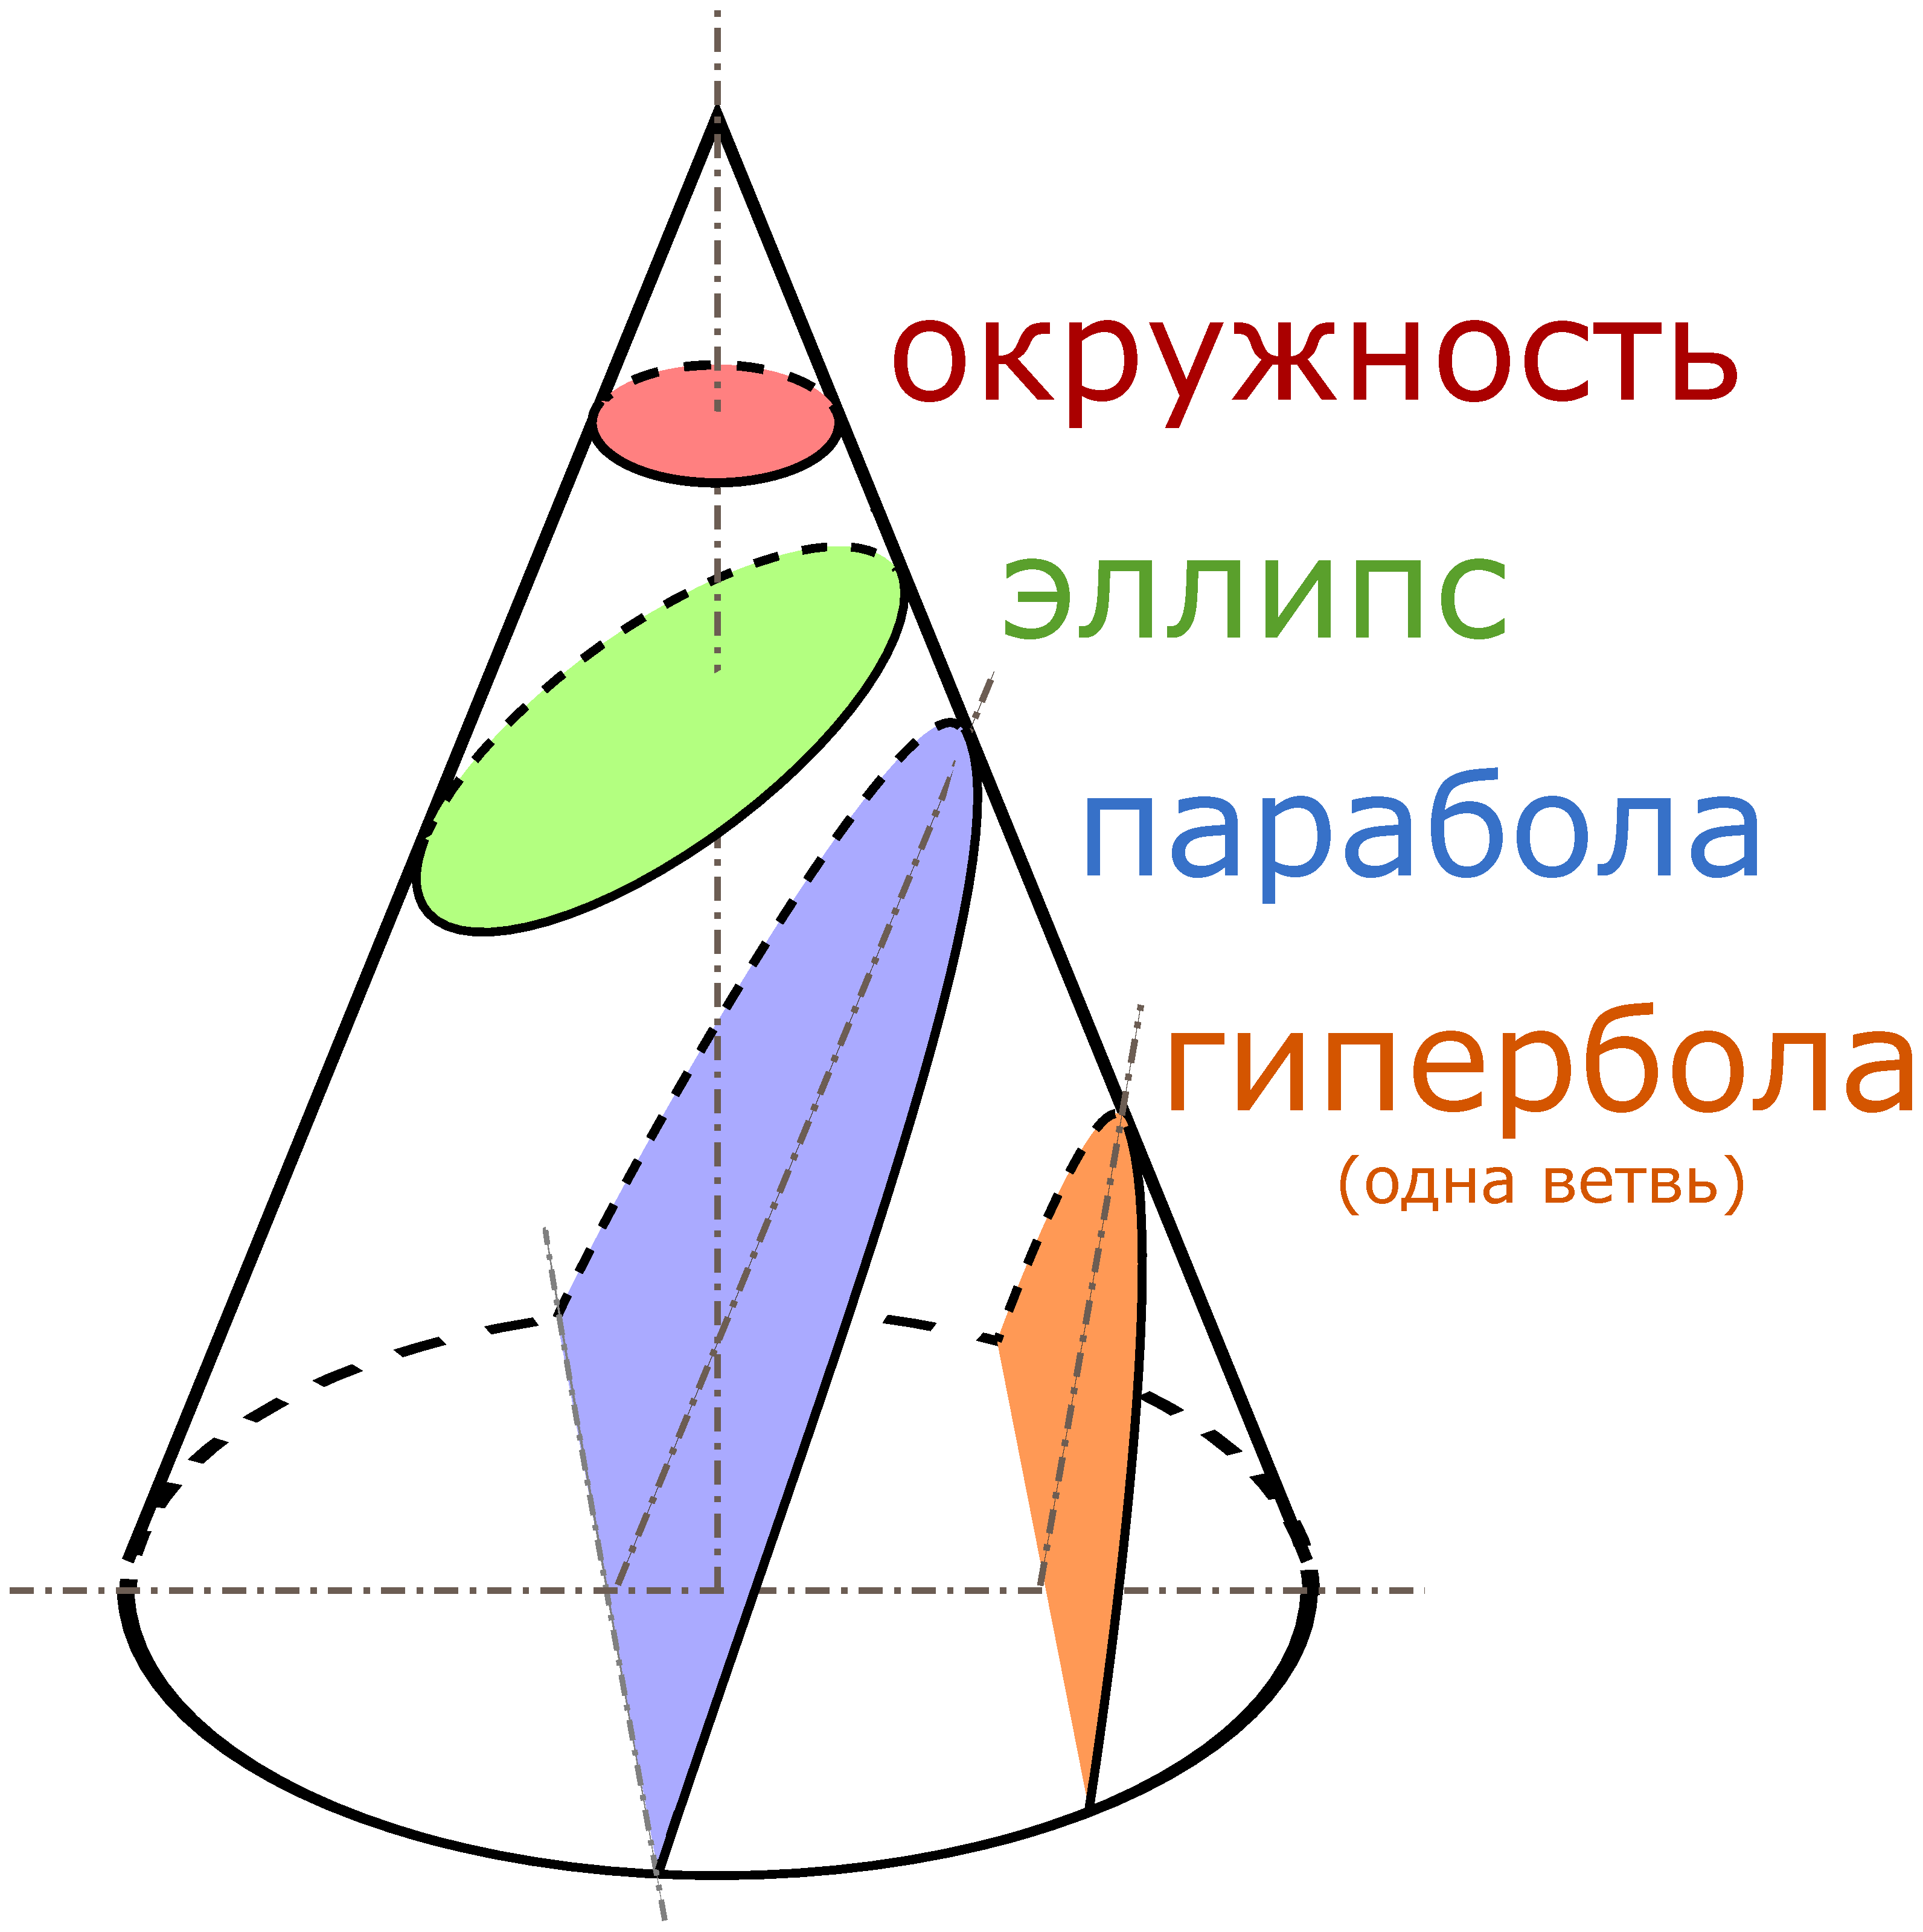
\includegraphics[width=0.4\textwidth]{conic_sections}
    
    \caption{Кривые второго порядка (эллипс, гипербола и парабола)~---~как конические сечения (\href{https://en.wikipedia.org/wiki/Conic_section}{wikipedia.org/wiki/Conic\_section}).}
    \label{fig:conic_sections}
  \end{figure}
  
  Можно заметить, что эксцентриситет увеличивается в ряду ``окружность, эллипс, парабола, гипербола'' (\ref{fig:eccentricity}).
  Таким образом, эксцентриситет выражает некую меру кривизны кривой: от максимальной у окружности до минимальной у гиперболы.

  \begin{figure}[h]
    \centering
    
    \begin{minipage}[c]{0.4\textwidth}  % https://tex.stackexchange.com/a/29163/135045
      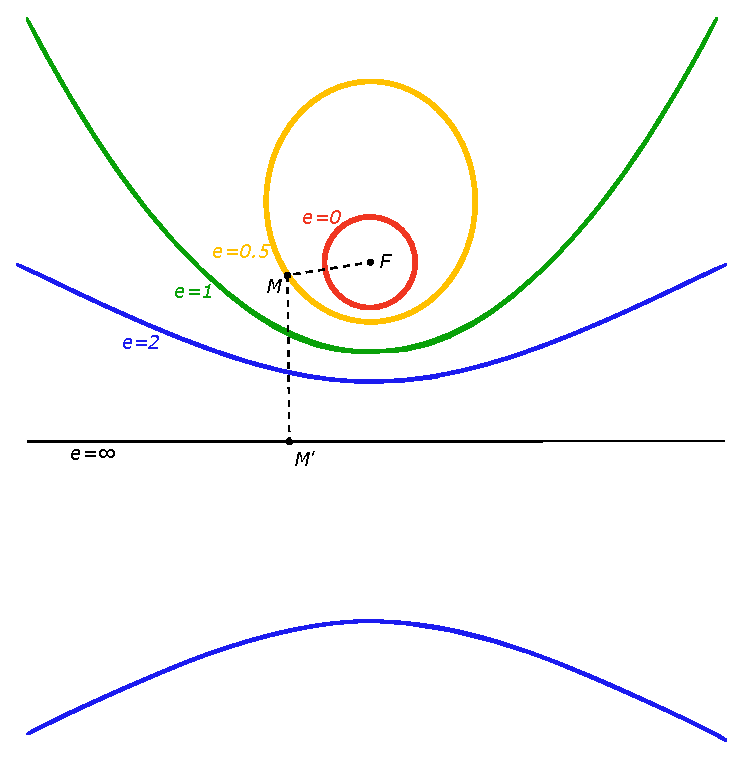
\includegraphics[width=\textwidth]{eccentricity}
    \end{minipage}\hfill
    \begin{minipage}[c]{0.55\textwidth}
      \caption{Эксцентриситет~---~как число, отражающее кривизну линии второго порядка (\href{https://en.wikipedia.org/wiki/Conic_section}{wikipedia.org/wiki/Conic\_section}). Кривизна уменьшается с увеличением эксцентриситета.}
      \label{fig:eccentricity}
    \end{minipage}
  \end{figure}
  
  
  Мы определяли эксцентриситет для эллипса и гиперболы через отношение $c$ к $a$ (к слову,  $c$ ещё называют \emph{линейным эксцентриситетом} или \emph{фокальным расстоянием}~---~расстояние между центром и фокусом).
  У параболы же нет $c$ (так как нет центра), но у неё эксцентриситет был равен одному как отношение расстояние от точки параболы до фокуса к расстоянию от той же точки до директрисы.
  Существует более общее определение эксцентриситета, которое подходит как для окружности, так и для эллипса, гиперболы и параболы~---~через конические сечения (\ref{fig:eccentricity_definition}):
  \[
    \left\{
      \begin{aligned}
        &\eps = \frac{\sin \beta}{\sin \alpha}\\
        &0 < \alpha < \frac{\pi}{2}\\
        &0 \leq \beta \leq \frac{\pi}{2}
      \end{aligned}
    \right.
  \]
  где $\beta$~---~угол наклона секущей конус плоскости, а $\alpha$~---~угол между образующей конуса и его основанием.
  
  В пределе $\alpha \hm\to +\infty$ (сплющенный конус) в сечении в пределе получается прямая, поэтому для прямой можно считать эксцентриситет $\eps \hm\to +\infty$ (\ref{fig:eccentricity}).
  
  
  \begin{figure}[h]
    \centering
    
    \begin{minipage}[c]{0.25\textwidth}
      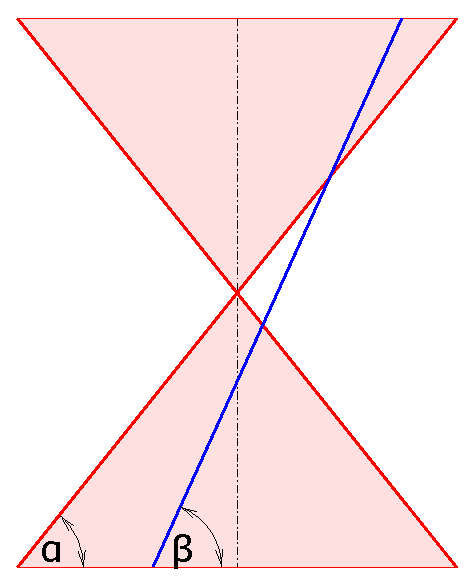
\includegraphics[width=\textwidth]{eccentricity_definition}
    \end{minipage}\hfill
    \begin{minipage}[c]{0.75\textwidth}
      \caption{К определению эксцентриситета через конические сечения (\href{https://en.wikipedia.org/wiki/Eccentricity_(mathematics)}{wikipedia.org/wiki/Eccentricity}).}
      \label{fig:eccentricity_definition}
    \end{minipage}
  \end{figure}
  
  
  \subsection{Про $2p$}
  
  В каноническом уравнении параболы
  \[
    y^2 = 2px,\quad p > 0
  \]
  двойка на самом деле ``не просто так'': $p$~---~половина так называемого \emph{latus rectum}\footnote{Latus переводится с латинского как ``прямой'', а rectum~---~``кишка''?.. Или это всё вместе переводится как ``прямая сторона'' (по другим источникам)?.. Автор конспекта доунт ноу.} (\ref{fig:semi_latus_rectum}).
  То есть $p$~---~это длина части перпендикуляра к оси параболы, проходящего через фокус, от фокуса до параболы.
  Точно так же $p$ определяется и в случае эллипса и гиперболы.
  
  \begin{figure}[h]
    \centering

    \begin{minipage}[c]{0.4\textwidth}
      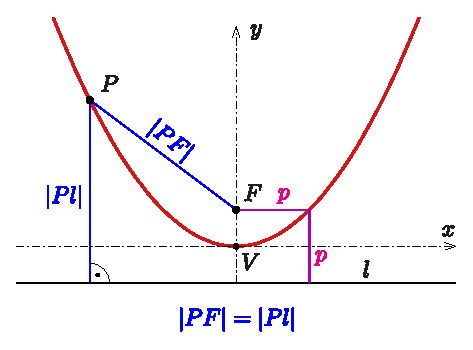
\includegraphics[width=\textwidth]{semi_latus_rectum}
    \end{minipage}\hfill
    \begin{minipage}[c]{0.55\textwidth}
      \caption{Число $p$ из канонического уравнения параболы (\href{https://en.wikipedia.org/wiki/Parabola}{wikipedia.org/wiki/Parabola}).}
      \label{fig:semi_latus_rectum}
    \end{minipage}
  \end{figure}
\end{document}
